%
% A header that lets you compile a chapter by itself, or inside a larger document.
% Adapted from stackoverflow.com/questions/3655454/conditional-import-in-latex
%
%
%Use \inbpdocument and \outbpdocument in your individual files, in place of \begin{document} and \end{document}. In your main file, put in a \def \ismaindoc {} before including or importing anything.
%
% David Duvenaud
% June 2011
% 
% ======================================
%
%


\ifx\ismaindoc\undefined
	\newcommand{\inbpdocument}{
		\def \ismaindoc {}
		% Use this header if we are compiling by ourselves.
		\documentclass[a4paper,11pt,authoryear,index]{common/PhDThesisPSnPDF}
		
%\usepackage{draftwatermark}
%\SetWatermarkLightness{0.95}

% ******************************************************************************
% ****************************** Custom Margin *********************************

% Add `custommargin' in the document class options to use this section
% Set {innerside margin / outerside margin / topmargin / bottom margin}  and
% other page dimensions

\ifsetMargin
\else
    \RequirePackage[left=37mm,right=30mm,top=35mm,bottom=30mm]{geometry}
    \setFancyHdr % To apply fancy header after geometry package is loaded
\fi


%\chead{Unfinished draft}
%\cfoot{\texttt{Unfinished draft - compiled on \today{} at \currenttime}}

% *****************************************************************************
% ******************* Fonts (like different typewriter fonts etc.)*************

% Add `customfont' in the document class option to use this section

\ifsetFont
\else
    % Set your custom font here and use `customfont' in options. Leave empty to
    % load computer modern font (default LaTeX font).  

    \RequirePackage{libertine} 
\fi

% *****************************************************************************
% *************************** Bibliography  and References ********************

%\usepackage{cleveref} %Referencing without need to explicitly state fig /table

% Add `custombib' in the document class option to use this section
\ifsetBib % True, Bibliography option is chosen in class options
\else % If custom bibliography style chosen then load bibstyle here

   \RequirePackage[square, sort, numbers, authoryear]{natbib} % CustomBib

% If you would like to use biblatex for your reference management, as opposed to the default `natbibpackage` pass the option `custombib` in the document class. Comment out the previous line to make sure you don't load the natbib package. Uncomment the following lines and specify the location of references.bib file

% \RequirePackage[backend=biber, style=numeric-comp, citestyle=numeric, sorting=nty, natbib=true]{biblatex}
% \bibliography{References/references} %Location of references.bib only for biblatex

\fi


% changes the default name `Bibliography` -> `References'
\renewcommand{\bibname}{References}


% *****************************************************************************
% *************** Changing the Visual Style of Chapter Headings ***************
% Uncomment the section below. Requires titlesec package.

%\RequirePackage{titlesec}
%\newcommand{\PreContentTitleFormat}{\titleformat{\chapter}[display]{\scshape\Large}
%{\Large\filleft{\chaptertitlename} \Huge\thechapter}
%{1ex}{}
%[\vspace{1ex}\titlerule]}
%\newcommand{\ContentTitleFormat}{\titleformat{\chapter}[display]{\scshape\huge}
%{\Large\filleft{\chaptertitlename} \Huge\thechapter}{1ex}
%{\titlerule\vspace{1ex}\filright}
%[\vspace{1ex}\titlerule]}
%\newcommand{\PostContentTitleFormat}{\PreContentTitleFormat}
%\PreContentTitleFormat


% *****************************************************************************
% **************************** Custom Packages ********************************
% *****************************************************************************


% ************************* Algorithms and Pseudocode **************************

%\usepackage{algpseudocode} 


% ********************Captions and Hyperreferencing / URL **********************

% Captions: This makes captions of figures use a boldfaced small font. 
%\RequirePackage[small,bf]{caption}

\RequirePackage[labelsep=space,tableposition=top]{caption} 
%\renewcommand{\figurename}{Figure} %to support older versions of captions.sty
\captionsetup{labelsep = colon,belowskip=12pt,aboveskip=4pt}

% ************************ Formatting / Footnote *******************************

%\usepackage[perpage]{footmisc} %Range of footnote options 


% ****************************** Line Numbers **********************************

%\RequirePackage{lineno}
%\linenumbers

% ************************** Graphics and figures *****************************

%\usepackage{rotating}
%\usepackage{wrapfig}
%\usepackage{float}
\usepackage{subfig} %note: subfig must be included after the `caption` package. 


% ********************************* Table **************************************

%\usepackage{longtable}
%\usepackage{multicol}
%\usepackage{multirow}
%\usepackage{tabularx}


% ***************************** Math and SI Units ******************************

\usepackage{amsfonts}
\usepackage{amsmath}
\usepackage{amssymb}
%\usepackage{siunitx} % use this package module for SI units


% ******************************************************************************
% ************************* User Defined Commands ******************************
% ******************************************************************************

% *********** To change the name of Table of Contents / LOF and LOT ************

%\renewcommand{\contentsname}{My Table of Contents}
%\renewcommand{\listfigurename}{List of figures}
%\renewcommand{\listtablename}{List of tables}


% ********************** TOC depth and numbering depth *************************

\setcounter{secnumdepth}{2}
\setcounter{tocdepth}{2}

% ******************************* Nomenclature *********************************

% To change the name of the Nomenclature section, uncomment the following line

%\renewcommand{\nomname}{Symbols}


% ********************************* Appendix ***********************************

% The default value of both \appendixtocname and \appendixpagename is `Appendices'. These names can all be changed via: 

%\renewcommand{\appendixtocname}{List of appendices}
%\renewcommand{\appendixname}{Appndx}

		% All my custom preamble stuff.  Shouldn't overlap with anything in official-preamble




% Paths to figure and table directories.
\newcommand{\symmetryfigsdir}{figures/symmetries}
\newcommand{\topologyfiguresdir}{figures/topology}
\newcommand{\infinitefiguresdir}{figures/infinite}
\newcommand{\grammarfiguresdir}{figures/grammar}
\newcommand{\introfigsdir}{figures/intro}
\newcommand{\gplvmfiguresdir}{figures/gplvm}
\newcommand{\warpedfiguresdir}{figures/warped-mixtures}
\newcommand{\deeplimitsfiguresdir}{figures/deep-limits}
\newcommand{\quadraturefigsdir}{figures/quadrature}
\newcommand{\additivefigsdir}{figures/additive}
\newcommand{\decompfigsdir}{figures/decomp}
\newcommand{\examplefigsdir}{figures/worked-example}

\usepackage{bm}  % for warped mixtures - is this necessary?
\usepackage{booktabs}
\usepackage{tabularx}
\usepackage{multirow}
\usepackage{datetime}
\renewcommand{\tabularxcolumn}[1]{>{\arraybackslash}m{#1}}
\usepackage{relsize}
\usepackage{graphicx}
\usepackage{amsmath,amssymb,textcomp}
\usepackage{nicefrac}
\usepackage{amsthm}
\usepackage{tikz}
\usetikzlibrary{arrows}
\usetikzlibrary{calc}
\usepackage{nth}
\usepackage{rotating}
\usepackage{array}
\usepackage{fp}
\usepackage{cleveref}   % Note: this package sometimes causes the page counter to reset.
\crefname{equation}{equation}{equations}
\crefname{figure}{figure}{figures}
%\usepackage{common/sectsty}

% Controls capitalization of all headers
%\usepackage{stringstrings}
%\usepackage[explicit]{titlesec}
%\newcommand\SentenceCase[1]{%
%  \caselower[e]{#1}%
%  \capitalize[q]{\thestring}%
%}
%\titleformat{\section}
%  {\normalfont\Large\bfseries}{\thesection}{1em}{\SentenceCase{#1}\thestring}


%\titleformat{\section} % The normal, unstarred version
%    {\Large\bfseries}{}{2ex}
%    {\thesection. \MakeSentenceCase{#1}}

%\titleformat{name=\section,numberless} % The starred version; note the `numberless` key
%    {\Large\bfseries}{}{2ex}
%    {\MakeSentenceCase{#1}}

\usepackage[hyperpageref]{backref}
% Setup to show (pages 4 and 9) sort of thing in the bibliography - DD
%\def\foo{\hspace{\fill}\mbox{}\linebreak[0]\hspace*{\fill}}
%\def\foo{\parbox{3cm}{\hfill}
%\def\foo{\parbox{3cm}{\hfill}
%\newcommand\foo[1]{{\raggedleft{\hfill{\mbox{\hfill{#1}}}}}}
\newcommand{\comfyfill}[1]{% = Thorsten Donig's \signed
  \unskip\hspace*{0.1em plus 1fill}
  \nolinebreak[3]%
  \hspace*{\fill}\mbox{#1}
  \parfillskip0pt\par
}
\newcommand\foo[1]{{\comfyfill{\mbox{#1}}}}
%\newcommand\foo[1]{{\mbox{#1}}}
\renewcommand*{\backref}[1]{}
\renewcommand*{\backrefalt}[4]{%
\ifcase #1 %
%
\or
\foo{(page #2)}%
\else
\foo{(pages #2)}%
\fi
}

\usepackage{stringstrings}

%\newcommand{\headercase}{\
%\DeclareFieldFormat{titlecase}{\MakeSentenceCase{#1}}


%% For submission, make all render blank.
%%%%%%%%%%%%%%%%%%%%%%%%%%%%%%%%%%%%%%%%%%%%%%%%%%%%%%%%%%
%%%% EDITING HELPER FUNCTIONS  %%%%%%%%%%%%%%%%%%%%%%%%%%%
%%%%%%%%%%%%%%%%%%%%%%%%%%%%%%%%%%%%%%%%%%%%%%%%%%%%%%%%%%

%% NA: needs attention (rough writing whose correctness needs to be verified)
%% TBD: instructions for how to fix a gap ("Describe the propagation by ...")
%% PROBLEM: bug or missing crucial bit 

%% use \fXXX versions of these macros to put additional explanation into a footnote.  
%% The idea is that we don't want to interrupt the flow of the paper or make it 
%% impossible to read because there are a bunch of comments.

%% NA's (and TBDs, those less crucially) should be written so 
%% that they flow with the text.

\definecolor{WowColor}{rgb}{.75,0,.75}
\definecolor{SubtleColor}{rgb}{0,0,.50}

% inline
\newcommand{\NA}[1]{\textcolor{SubtleColor}{ {\tiny \bf ($\star$)} #1}}
\newcommand{\LATER}[1]{\textcolor{SubtleColor}{ {\tiny \bf ($\dagger$)} #1}}
\newcommand{\TBD}[1]{\textcolor{SubtleColor}{ {\tiny \bf (!)} #1}}
\newcommand{\PROBLEM}[1]{\textcolor{WowColor}{ {\bf (!!)} {\bf #1}}}

% as margin notes

\newcounter{margincounter}
\newcommand{\displaycounter}{{\arabic{margincounter}}}
\newcommand{\incdisplaycounter}{{\stepcounter{margincounter}\arabic{margincounter}}}

\newcommand{\fTBD}[1]{\textcolor{SubtleColor}{$\,^{(\incdisplaycounter)}$}\marginpar{\tiny\textcolor{SubtleColor}{ {\tiny $(\displaycounter)$} #1}}}

\newcommand{\fPROBLEM}[1]{\textcolor{WowColor}{$\,^{((\incdisplaycounter))}$}\marginpar{\tiny\textcolor{WowColor}{ {\bf $\mathbf{((\displaycounter))}$} {\bf #1}}}}

\newcommand{\fLATER}[1]{\textcolor{SubtleColor}{$\,^{(\incdisplaycounter\dagger)}$}\marginpar{\tiny\textcolor{SubtleColor}{ {\tiny $(\displaycounter\dagger)$} #1}}}

%\renewcommand{\LATER}[1]{}
%\renewcommand{\fLATER}[1]{}
%\renewcommand{\TBD}[1]{}
%\renewcommand{\fTBD}[1]{}
%\renewcommand{\PROBLEM}[1]{}
%\renewcommand{\fPROBLEM}[1]{}
%\renewcommand{\NA}[1]{}


% HUMBLE WORDS: shown slightly smaller when in normal text
% Thanks to Christian Steinruecken!

% HUMBLE WORDS: shown slightly smaller when in normal text
% Christian Steinruecken
%
\makeatletter%
%\def\@humbleformat#1{{\fontsize{}{1em}\selectfont #1}}
%\def\@humbleformat#1{\textsmaller{#1}}%
\newlength{\nonHumbleHeight}
\def\@humbleformat#1{{\settoheight{\nonHumbleHeight}{#1}\resizebox{!}{0.94\nonHumbleHeight}{#1}}}%
\def\@idxhumbleformat#1{{\relscale{0.95}{#1}}}%
%\def\@humbleformat#1{{#1}}%
\def\declareHumble#1#2{%
  \expandafter\def\csname #1\endcsname{\@humbleformat{#2}}%
  \expandafter\def\csname s#1\endcsname{{#2}}%
  \expandafter\def\csname idx#1\endcsname{{\@idxhumbleformat{#2}}}%
}%
\def\humble#1{\@humbleformat{#1}}%
\def\idxhumble#1{\@idxhumbleformat{#1}}%
\makeatother%

% Convenient indexing for humble abbreviations
\def\humbleindex#1#2{\index{#1@\idxhumble{#1}}}



% TODO: Clean up duplicates
\declareHumble{ANOVA}{ANOVA}
\declareHumble{ARD}{ARD}
\declareHumble{BIC}{BIC}
\declareHumble{BMC}{BMC}
\declareHumble{bq}{BQ}
\declareHumble{CRP}{CRP}
\declareHumble{dirpro}{DP}
\declareHumble{HDMR}{HDMR}
\declareHumble{GAM}{GAM}
\declareHumble{GEM}{GEM}
\declareHumble{GMM}{GMM}
\declareHumble{gplvm}{GP-LVM}
\declareHumble{gpml}{GPML}
\declareHumble{GPML}{GPML}
\declareHumble{gprn}{GPRN}
\declareHumble{gpt}{GP}
\declareHumble{gp}{GP}
\declareHumble{HKL}{HKL}
\declareHumble{HMC}{HMC}
\declareHumble{ibp}{IBP}
\declareHumble{iGMM}{iGMM}
\declareHumble{iwmm}{iWMM}
\declareHumble{kCP}{CP}
\declareHumble{kCW}{CW}
\declareHumble{kC}{C}
\declareHumble{KDE}{KDE}
\declareHumble{kLin}{Lin}
\declareHumble{KPCA}{KPCA}
\declareHumble{kPer}{Per}
\declareHumble{kPerGen}{ZMPer}
\declareHumble{kRQ}{RQ}
\declareHumble{kSE}{SE}
\declareHumble{kWN}{WN}
\declareHumble{Lin}{Lin}
\declareHumble{LBFGS}{L-BFGS}
\declareHumble{LIBSVM}{LIBSVM}
\declareHumble{MAP}{MAP}
\declareHumble{mcmc}{MCMC}
\declareHumble{MKL}{MKL}
\declareHumble{MLP}{MLP}
\declareHumble{MNIST}{MNIST}
\declareHumble{MSE}{MSE}
\declareHumble{OU}{OU}
\declareHumble{Per}{Per}
\declareHumble{RBF}{RBF}
\declareHumble{RMSE}{RMSE}
\declareHumble{RQ}{RQ}
\declareHumble{SBQ}{SBQ}
\declareHumble{seard}{SE-ARD}
\declareHumble{sefull}{SE-\textnormal{full}}
\declareHumble{SEGP}{SE-GP}
\declareHumble{SE}{SE}
\declareHumble{SNR}{SNR}
\declareHumble{SSANOVA}{SS-ANOVA}
\declareHumble{SVM}{SVM}
\declareHumble{UCI}{UCI}
\declareHumble{UMIST}{UMIST}
\declareHumble{vbgplvm}{VB GP-LVM}

\newcommand{\kSig}{\boldsymbol\sigma}

\def\subexpr{{\cal S}}
\def\baseker{{\cal B}}
\def\numWinners{k}

\def\ie{i.e.\ }
\def\eg{e.g.\ }
\def\etc{etc.\ }
\let\oldemptyset\emptyset
%\let\emptyset 0




% Unify notation between neural-net land and GP-land.
\newcommand{\hphi}{h}
\newcommand{\hPhi}{\vh}
\newcommand{\walpha}{w}
\newcommand{\wboldalpha}{\bw}
\newcommand{\wcapalpha}{\vW}
\newcommand{\lengthscale}{w}

\newcommand{\layerindex}{\ell}



\newcommand{\gpdrawbox}[1]{
\setlength\fboxsep{0pt}
\hspace{-0.15in} 
\fbox{
\includegraphics[width=0.464\columnwidth]{\deeplimitsfiguresdir/deep_draws/deep_gp_sample_layer_#1}
}}



\newcommand{\procedurename}{ABCD}
\newcommand{\genText}[1]{{\sf #1}}



\newcommand{\asdf}{$^{\textnormal{th}}$}

\newcommand{\binarysum}{\sum_{\bf{x} \in \{0,1\}^D}}
\newcommand{\expect}{\mathbb{E}}
\newcommand{\expectargs}[2]{\mathbb{E}_{#1} \left[ {#2} \right]}
\newcommand{\var}{\mathbb{V}}
\newcommand{\varianceargs}[2]{\mathbb{V}_{#1} \left[ {#2} \right]}
\newcommand{\cov}{\operatorname{cov}}
\newcommand{\Cov}{\operatorname{Cov}}
\newcommand{\covargs}[2]{\Cov \left[ {#1}, {#2} \right]}
\newcommand{\variance}{\mathbb{V}}
\newcommand{\vecop}[1]{\operatorname{vec} \left( {#1} \right)}

\newcommand{\covarianceargs}[2]{\Cov_{#1} \left[ {#2} \right]}
\newcommand{\colvec}[2]{\left[ \begin{array}{c} {#1} \\ {#2} \end{array} \right]}
\newcommand{\tbtmat}[4]{\left[ \begin{array}{cc} {#1} & {#2} \\ {#3} & {#4} \end{array} \right]}

\newcommand{\acro}[1]{{\humble{#1}}}
%\newcommand{\vect}[1]{\boldsymbol{#1}}
\newcommand{\vect}[1]{{\bf{#1}}}
\newcommand{\mat}[1]{\mathbf{#1}}
\newcommand{\pderiv}[2]{\frac{\partial #1}{\partial #2}}
\newcommand{\npderiv}[2]{\nicefrac{\partial #1}{\partial #2}}

\newcommand{\pha}{^{\phantom{:}}}

\newcommand{\argmin}{\operatornamewithlimits{argmin}}
\newcommand{\argmax}{\operatornamewithlimits{argmax}}

% The following designed for probabilities with long arguments

\newcommand{\Prob}[2]{P\!\left(\,#1\;\middle\vert\;#2\,\right)}
\newcommand{\ProbF}[3]{P\!\left(\,#1\!=\!#2\;\middle\vert\;#3\,\right)}
\newcommand{\p}[2]{p\!\left(#1\middle\vert#2\right)}
\newcommand{\po}[1]{p\!\left(#1\right)}
\newcommand{\pF}[3]{p\!\left(\,#1\!=\!#2\;\middle\vert\;#3\,\right)} 
\newcommand{\mean}[2]{{m}\!\left(#1\middle\vert#2\right)}



\newcommand{\valpha}{\boldsymbol{\alpha}}
\newcommand{\va}{\vect{a}}
\newcommand{\vA}{\vect{A}}
\newcommand{\vB}{\mat{B}}
\newcommand{\vb}{\vect{b}}
\newcommand{\vC}{\mat{C}}
\newcommand{\vc}{\vect{c}}
\newcommand{\vecf}{\boldsymbol{f}}
\newcommand{\vell}{\vect{\ell}}
\newcommand{\vepsilon}{\boldsymbol{\epsilon}}
\newcommand{\veps}{\boldsymbol{\epsilon}}
\newcommand{\ve}{\boldsymbol{\epsilon}}
\newcommand{\vf}{\vecf}
\newcommand{\vg}{\vect{g}}
\newcommand{\vh}{\vect{h}}
\newcommand{\vI}{\mat{I}}
\newcommand{\vK}{\mat{K}}
\newcommand{\vk}{\vect{k}}
\newcommand{\vL}{\mat{L}}
\newcommand{\vl}{\vect{l}}
\newcommand{\vmu}{{\boldsymbol{\mu}}}
\newcommand{\vone}{\vect{1}}
\newcommand{\vphi}{{\boldsymbol{\phi}}}
\newcommand{\vpi}{{\boldsymbol{\pi}}}
\newcommand{\vq}{\vect{q}}
\newcommand{\vR}{\mat{R}}
\newcommand{\vr}{\vect{r}}
\newcommand{\vsigma}{{\boldsymbol{\sigma}}}
\newcommand{\vSigma}{\mat{\Sigma}}
\newcommand{\vS}{\mat{S}}
\newcommand{\vs}{\vect{s}}
\newcommand{\vtheta}{{\boldsymbol{\theta}}}
\newcommand{\vu}{\vect{u}}
\newcommand{\vV}{\mat{V}}
\newcommand{\vW}{\mat{W}}
\newcommand{\vw}{\vect{w}}
\newcommand{\vX}{\mat{X}}
\newcommand{\vx}{\vect{x}}
\newcommand{\vY}{\mat{Y}}
\newcommand{\vy}{\vect{y}}
\newcommand{\vzero}{\vect{0}}
\newcommand{\vZ}{\mat{Z}}
\newcommand{\vz}{\vect{z}}


% deep gp notation
\newcommand{\netweights}{w}
\newcommand{\vnetweights}{\vw}
\newcommand{\mnetweights}{\vW}
\newcommand{\outweights}{\v}
\newcommand{\voutweights}{\vv}
\newcommand{\moutweights}{\vV}

\newcommand{\unitparams}{\v}
\newcommand{\vunitparams}{\vv}
\newcommand{\munitparams}{\vV}


\newcommand{\He}{\mathcal{H}}
\newcommand{\normx}[2]{\left\|#1\right\|_{#2}}
\newcommand{\Hnorm}[1]{\normx{#1}{\He}}
\newcommand{\mmd}{{\rm MMD}}


\newcommand{\mf}{\bar{\vf}}

%\newcommand{\mf}{\mu} %{\bar{\ell}}
\newcommand{\lf}{f} % Likelihood function
\newcommand{\st}{_\star}

% from simpler log-bq writeup
\newcommand{\lftwo}{{\log \ell}}
\newcommand{\mftwo}{{\bar \ell}}
\newcommand{\loggp}{{\log\acro{GP}}}%| \bX, \vy )}}
\newcommand{\loggpdist}{{\acro{GP}(\lftwo)}}%| \vX, \vy )}}


\newcommand{\inv}{^{{\mathsmaller{-1}}}}
\newcommand{\tohalf}{^{{\mathsmaller{\nicefrac{1}{2}}}}}

\newcommand{\Normal}{\mathcal{N}}
\newcommand{\N}[3]{\mathcal{N}\!\left(#1 \middle| #2,#3\right)}
\newcommand{\Nt}[2]{\mathcal{N}\!\left(#1,#2\right)}
\newcommand{\NT}[2]{\mathcal{N}\!\left(#1,#2\right)}
\newcommand{\GPdist}[3]{\mathcal{GP}\!\left(#1 \, \middle| \, #2, #3 \right)}
\newcommand{\GPdisttwo}[2]{\mathcal{GP}\!\left(\, #1, #2 \right)}
\newcommand{\bN}[3]{\mathcal{N}\big(#1 \middle| #2,#3\big)}
\newcommand{\boldN}[3]{\text{\textbf{\mathcal{N}}}\big(#1;#2,#3\big)}
\newcommand{\ones}[1]{\mat{1}_{#1}}
\newcommand{\eye}[1]{\mat{E}_{#1}}
\newcommand{\tra}{^{\mathsf{T}}}
%\newcommand{\tra}{^{\top}}
%\mathsf{T}
\newcommand{\trace}{\operatorname{tr}}
\newcommand{\shift}{\operatorname{shift}}
\renewcommand{\mod}{\operatorname{mod}}
\newcommand{\deq}{:=}
\newcommand{\oneofk}{\operatorname{one-of-k}}
%\newcommand{\degree}{^\circ}

\newcommand{\GPt}[2]{\mathcal{GP}\!\left(#1,#2\right)}
%\newcommand{\GPt}[2]{\gp\!\left(#1,#2\right)}

\DeclareMathOperator{\tr}{tr}
\DeclareMathOperator{\chol}{chol}
\DeclareMathOperator{\diag}{diag}

\newenvironment{narrow}[2]{%
  \begin{list}{}{%
  \setlength{\topsep}{0pt}%
  \setlength{\leftmargin}{#1}%
  \setlength{\rightmargin}{#2}%
  \setlength{\listparindent}{\parindent}%
  \setlength{\itemindent}{\parindent}%
  \setlength{\parsep}{\parskip}}%
\item[]}{\end{list}}



\newcommand{\dist}{\ \sim\ }
\def\given{\,|\,}

% Table stuff
\newcolumntype{C}[1]{>{\centering\let\newline\\\arraybackslash\hspace{0pt}}m{#1}}
\newcolumntype{L}[1]{>{\raggedright\let\newline\\\arraybackslash\hspace{0pt}}m{#1}}
\newcolumntype{R}[1]{>{\raggedleft\let\newline\\\arraybackslash\hspace{0pt}}m{#1}}

\newcommand{\defeq}{\mathrel{:\mkern-0.25mu=}}

\def\ie{i.e.\ }
\def\eg{e.g.\ }
\def\iid{i.i.d.\ }
%\def\simiid{\sim_{\mbox{\tiny iid}}}
\def\simiid{\overset{\mbox{\tiny iid}}{\sim}}
\def\simind{\overset{\mbox{\tiny \textnormal{ind}}}{\sim}}
\def\eqdist{\stackrel{\mbox{\tiny d}}{=}}
%\newcommand{\distas}[1]{\mathbin{\overset{#1}{\kern \z@ \sim}}}
%TODO: fix this - it worked outside the thesis!
\newcommand{\distas}[1]{\mathbin{\overset{#1}{\sim}}}

\def\Reals{\mathbb{R}}

\def\Uniform{\mbox{\rm Uniform}}
\def\Bernoulli{\mbox{\rm Bernoulli}}
\def\GP{\mathcal{GP}}
\def\GPLVM{\mathcal{GP-LVM}}




% Kernel stuff

\def\iva{\vect{\inputVar}}
\def\ivaone{\inputVar}
\def\inputVar{x}
\def\InputVar{X}
\def\InputSpace{\mathcal{X}}
\def\outputVar{y}
\def\OutputSpace{\mathcal{Y}}
\def\function{f}
\def\kernel{k}
\def\KernelMatrix{K}
\def\SumKernel{\sum}
\def\ProductKernel{\prod}
\def\expression{e}
\def\feat{\vh}

\newcommand{\kerntimes}{ \! \times \!}
\newcommand{\kernplus}{ \, + \,}


% Proof stuff
\theoremstyle{plain}
\newtheorem{theorem}{Theorem}[section]
\newtheorem{lemma}[theorem]{Lemma}
\newtheorem{prop}[theorem]{Proposition}
\newtheorem{proposition}{Proposition}
\newtheorem*{cor}{Corollary}

% For infinite bq
\newcommand{\iv}{\theta}
\newcommand{\viv}{\vtheta}

% For intro chapter
\newcommand{\funcval}{\vf(\vX)}
\newcommand{\testpoint}{{\vx^\star}}

\newcommand{\underwrite}[2]{{\underbrace{#1}_{\textnormal{#2}}}}



% For kernel figures
\newcommand{\fhbig}{2cm}%
\newcommand{\fwbig}{3cm}%
\newcommand{\kernpic}[1]{\includegraphics[height=\fhbig,width=\fwbig]{\grammarfiguresdir/structure_examples/#1}}%
\newcommand{\kernpicr}[1]{\rotatebox{90}{\includegraphics[height=\fwbig,width=\fhbig]{\grammarfiguresdir/structure_examples/#1}}}%
\newcommand{\addkernpic}[1]{{\includegraphics[height=\fhbig,width=\fwbig]{\grammarfiguresdir/additive_multi_d/#1}}}%
\newcommand{\largeplus}{\tabbox{{\Large+}}}%
\newcommand{\largeeq}{\tabbox{{\Large=}}}%
\newcommand{\largetimes}{\tabbox{{\Large$\times$}}}%
\newcommand{\fixedx}{$x$ (with $x' = 1$)}%

% for warped mixtures
\newcommand{\CLAS}{\vz}  %cluster assignments
\newcommand{\CLASi}{z} % individual cluster assignments


		% ************************ Thesis Information & Meta-data **********************

%% The title of the thesis
\title{Automating statistical modelling}

%\texorpdfstring is used for PDF metadata. Usage:
%\texorpdfstring{LaTeX_Version}{PDF Version (non-latex)} eg.,
%\texorpdfstring{$sigma$}{sigma}

%% The full name of the author
\author{James Robert Lloyd}

%% Department (eg. Department of Engineering, Maths, Physics)
%\dept{Department of Engineering}

%% University and Crest
\university{University of Cambridge}
\crest{
\includegraphics[width=0.25\textwidth]{misc/University_Crest}}

%% You can redefine the submission text:
% Default as per the University guidelines: This dissertation is submitted for
% the degree of Doctor of Philosophy
%\renewcommand{\submissiontext}{change the default text here if needed}

%% Full title of the Degree 
\degree{Doctor of Philosophy}
 
%% College affiliation (optional)
\college{Trinity College}

%% Submission date
\degreedate{December 2014} 

%% Meta information
\subject{Machine Learning}
\keywords{{LaTeX} {PhD Thesis} {Engineering} {University of Cambridge} {Machine Learning} {Gaussian processes} {Time Series} {Model checking} {Model criticism} {Aldous--Hoover} {Networks}}



		\begin{document}
	}	
	\newcommand{\outbpdocument}[1]{
		% Fake chapters so references aren't broken
		\label{ch:intro}                
		\label{ch:dummy}
		\label{ch:discussion}
		%\bibliographystyle{common/CUEDthesis}
		\bibliographystyle{plainnat}
		\bibliography{references.bib}
		\end{document}
	}	
\else
	%If we're inside another document, no need to re-start the document.
	\ifx\inbpdocument\undefined
		\newcommand{\inbpdocument}{}
		\newcommand{\outbpdocument}[1]{}
	\fi
\fi

\inbpdocument

\chapter{Compositionally constructed kernels for Gaussian process models}
\label{ch:construction}

In the introduction we demonstrated that Gaussian processes can be used to express probability distributions over functions.
The properties of these distributions very much depended on the choice of kernel; different kernels where shown to yield probability distributions over smooth, linear and periodic functions.
In this chapter we address the problem of selecting which kernel to use in a Gaussian process model.
Our approach is to define an open ended space of potential kernel functions via a generative grammar and then perform model selection combined with a simple search strategy to explore the space of models.

This chapter is based upon joint work with David Duvenaud, Roger Grosse, Joshua Tenenbaum and Zoubin Ghahramani \citep{Duvenaud2013-dn}.
The initial ideas were formed during discussions between Roger, David and myself.
I performed the majority of experiments; all were involved with the writing.

\section{Introduction}

Kernel-based nonparametric models, such as support vector machines and Gaussian processes (\gp{}s), have been one of the dominant paradigms for supervised machine learning over the last 20 years.
These methods depend on defining a kernel function, $\kernel(\inputVar,\inputVar')$, which specifies how similar or correlated outputs $\outputVar$ and $\outputVar'$ are expected to be at two inputs $\inputVar$ and $\inputVar'$.
By defining the measure of similarity between inputs, the kernel determines the pattern of inductive generalisation.

%Most existing techniques pose kernel learning as a potentially high-dimensional parameter estimation problem.
%Examples include learning kernel parameters \cite{Rasmussen2006-ml}, linear combinations of fixed kernels \cite{Bach_HKL}, and mappings from the input space to an embedding space \cite{salakhutdinov2008using}.

However, to apply existing kernel learning algorithms, the user must typically specify the parametric form of the kernel, and this can require considerable expertise and / or several iterations of trial and error.

To make kernel learning more generally applicable we propose an automatic procedure to select an appropriate parametric form of a kernel.
In particular, we formulate a space of kernel structures defined compositionally in terms of sums and products of a small number of base kernels.
This produces an expressive modelling language which concisely captures many widely used techniques for constructing kernels.
We focus on Gaussian process regression, where the kernel specifies a covariance function, since the Bayesian framework provides natural methods by which to select between models.
Borrowing discrete search techniques which have proved successful in equation discovery \citep{Todorovski1997-st} and unsupervised learning \citep{Grosse2012-zi}, we automatically search over this space of kernel structures using model evidence as the search criterion.

We found that our kernel search algorithm is able to automatically recover known structures from synthetic data as well as plausible structures for a variety of real-world datasets. 
On a variety of time series datasets, the learned kernels yield decompositions of the unknown function into interpretable components that enable accurate extrapolation beyond the range of the observations.
Furthermore, the automatically discovered kernels outperform a variety of widely used kernel classes and kernel combination methods on supervised prediction tasks.

While we focus on Gaussian process regression, we believe our kernel search method can be extended to other supervised learning frameworks such as classification or ordinal regression, or to other kinds of kernel architectures such as kernel SVMs.
We hope that the algorithm developed in this chapter and the refinements made in chapter~\ref{ch:description} will help replace the current and often opaque art of kernel engineering with a more transparent science of automated kernel construction.

\section{Expressing high level patterns with kernels} 
\label{sec:construction:structure}

Gaussian process regression models use a kernel to define the covariance between any two function values: ${\textrm{Cov}(\outputVar, \outputVar') = \kernel(\inputVar,\inputVar')}$.
The kernel specifies which structures are likely under the \gp{} prior, which in turn determines the generalisation properties of the model.
In this section, we review the ways in which kernel families\footnotemark{} can be composed to express diverse probability distributions over functions. 
\footnotetext{When unclear from context, we use `kernel family' to refer to the parametric forms of the kernel functions. A kernel is a kernel family with all of the parameters specified.}  

There has been significant work on constructing kernels for use with Gaussian processes \citep[e.g. chapter 4 of][]{Rasmussen2006-ml}.
Commonly used kernel families include the squared exponential (\kSE)\footnotemark, periodic (\kPer), linear (\kLin), and rational quadratic (\kRQ) which are defined as follows:
\[
\kSE(\inputVar, \inputVar') =& \sigma^2\exp\left(-\frac{(\inputVar - \inputVar')^2}{2\ell^2}\right) \\
\kPer(\inputVar, \inputVar') =& \sigma^2\exp\left(-\frac{2\sin^2 (\pi(\inputVar - \inputVar')/p)}{\ell^2}\right) \\
\kLin(\inputVar, \inputVar') =& \sigma_b^2 + \sigma_v^2(\inputVar - \ell)(\inputVar' - \ell) \\
\kRQ(\inputVar, \inputVar') =& \sigma^2\left( 1 + \frac{(\inputVar - \inputVar')^2}{2 \alpha \ell^2} \right)^{-\alpha}
\]
\footnotetext{This kernel family is also known as the exponentiated quadratic and radial basis function.
I prefer the term exponentiated quadratic and recommend others to use it in future, but old habits die hard.}

\newcommand{\fhbig}{1.6cm}
\newcommand{\fwbig}{1.8cm}
\newcommand{\kernpic}[1]{\includegraphics[height=\fhbig,width=\fwbig]{\constructionfigsdir/structure_examples/#1}}
\newcommand{\kernpicr}[1]{\rotatebox{90}{\includegraphics[height=\fwbig,width=\fhbig]{\constructionfigsdir/structure_examples/#1}}}
\newcommand{\addkernpic}[1]{{\includegraphics[height=\fhbig,width=\fwbig]{\constructionfigsdir/additive_multi_d/#1}}}
\newcommand{\largeplus}{\tabbox{{\Large+}}}
\newcommand{\largeeq}{\tabbox{{\Large=}}}
\newcommand{\largetimes}{\tabbox{{\Large$\times$}}}
\begin{figure}[ht]
\centering
\renewcommand{\tabularxcolumn}[1]{>{\arraybackslash}m{#1}}
\begin{tabularx}{\columnwidth}{XXXX}
  \kernpic{se_kernel} & \kernpic{se_kernel_draws}
& \kernpic{per_kernel} & \kernpic{per_kernel_draws_s2}
\\
  {\small Squared \newline exponential (\kSE)} & {\small smooth} 
& {\small Periodic (\kPer)} & {\small periodic \newline and smooth}
\\
  \kernpic{lin_kernel} & \kernpic{lin_kernel_draws}
& \kernpic{rq_kernel} & \kernpic{rq_kernel_draws}
\\
  {\small Linear (\kLin)} & {\small linear \newline functions} 
& {\small Rational- \newline quadratic(\kRQ)} & {\small multi-scale \newline smoothness}
\end{tabularx}
\caption[Samples from Gaussian processes with differnet kernels.]{
Left and third columns: base kernels $k(\cdot,0)$.  Second and fourth columns: samples from a GP from each kernel.
The x-axis has the same range on all plots.}
\label{fig:basic_kernels}
\end{figure}

\paragraph{Composing Kernels}
Positive semidefinite kernels (\ie those which define valid covariance functions) are closed under addition and multiplication\footnotemark{}.
We can therefore use these two operations to create new kernels from old.
\footnotetext{And other operations \citep[e.g.][]{Rasmussen2006-ml}}

In particular, kernels over multidimensional inputs can be constructed by summation and multiplication of kernels acting on single dimensions of the input.
We therefore define our base kernel families to be one dimensional where we indicate the dimension the kernel applies to using subscripts e.g. $\SE_2$ represents an \kSE{} kernel over the second dimension of the input $\inputVar$.
%
\begin{figure}[ht]
\centering
\renewcommand{\tabularxcolumn}[1]{>{\arraybackslash}m{#1}}
\begin{tabularx}{\columnwidth}{XXXX}
  \kernpic{lin_times_lin} & \kernpic{lin_times_lin_draws} 
& \kernpic{se_times_per} & \kernpic{se_times_per_draws_s7}
\\
  {\small $\kLin \times \kLin$} & {\small quadratic}
& {\small $\kSE \times \kPer$} & {\small locally \newline periodic}
\\
  \kernpic{lin_plus_per} & \kernpic{lin_plus_per_draws}
& \kernpic{se_plus_per} & \kernpic{se_plus_per_draws_s7}
\\
  {\small $\kLin + \kPer$} & {\small periodic plus \newline linear trend}
& {\small $\kSE + \kPer$ } & {\small periodic plus \newline smooth trend}
\\
%  \kernpic{se_times_lin} & \kernpic{se_times_lin_draws_s2}
%& \kernpic{lin_times_per} & \kernpic{lin_times_per_draws_s2}
%\\
%  {\small $\kLin \times \kSE$} & {\small growing amplitude \newline smooth}
%& {\small $\kLin \times \kPer$} & {\small growing amplitude}
%\\
  \addkernpic{additive_kernel} & \addkernpic{additive_kernel_draw_sum}
& \addkernpic{sqexp_kernel}  & \addkernpic{sqexp_draw}
\\
  {\small $\kSE_1 + \kSE_2$} & {\small $f_1(x_1)$ $+$ $f_2(x_2)$}
& {\small $\kSE_1 \times \kSE_2$} & {\small $f(x_1, x_2)$}
\end{tabularx}
\caption[Samples from Gaussian processes with compositionally constructed kernels.]{Examples of structures expressible by
  composite kernels.  
  Left column and third columns: composite kernels $k(\cdot,0)$.
  Plots have the same meaning as in figure \ref{fig:basic_kernels}.}
\label{fig:kernels}
\end{figure}

\paragraph{Summation}

Suppose functions $\function_1$ and $\function_2$ are samples from independent \gp{} distributions, ${\function_1 \dist \gp{}(\mu_1, \kernel_1)}$, ${\function_2 \dist \gp{}(\mu_2, \kernel_2)}$.
Then ${\function \defas \function_1 + \function_2 \dist \gp{}(\mu_1 + \mu_2, \kernel_1 + \kernel_2)}$.
This allows us to create kernels that encode for distributions over superpositions of independent functions with different properties.

In a single dimension, sums of functions / kernels can express superposition of different processes, possibly operating at different scales.
In multiple dimensions, summing kernels gives additive structure over different dimensions, similar to generalized additive models~\citep{Hastie1990-ay}.
These two kinds of structure are demonstrated in rows 2 and 3 of figure~\ref{fig:kernels}, respectively.

\paragraph{Multiplication}

Multiplying kernels allows us to account for interactions between different input dimensions or different notions of similarity. 
For example, for multidimensional data, the multiplicative kernel $\SE_1 \times \SE_3$ encodes for a distribution over functions that vary smoothly with input dimensions 1 and 3 but is not constrained to be additive.
In one dimension, multiplying a kernel by \kSE{} removes any long range correlations in the distribution it encodes for.
For example, $\Per$ corresponds to globally periodic structure, whereas $\Per \times \SE$ corresponds to locally periodic structure, as shown in row 1 of figure~\ref{fig:kernels}.
This is made more precise in chapter~\ref{ch:description}.

Many architectures for learning complex functions, such as convolutional neural networks \citep[e.g.][]{LeCun1989-ba} or sum-product networks \citep{Poon2011-sc}, include units which compute AND-like and OR-like operations.
The composite kernels defined here can be viewed similarly.
A sum of kernels can be understood as an OR-like operation: two points are considered similar if either kernel has a high value.
Similarly, multiplying kernels is an AND-like operation, since two points are considered similar only if both kernels have high values.
Since we are applying these operations to the similarity functions rather than the regression functions themselves, compositions of even a few base kernels are able to capture complex relationships in data which do not have a simple parametric form.

\paragraph{Example expressions}

In addition to the examples given in figure~\ref{fig:kernels}, many common motifs of supervised learning can be captured using sums and products of one-dimensional base kernels:

\begin{tabular}{l|l}
Bayesian linear regression & $\Lin$ \\
Bayesian polynomial regression & $\Lin \times \Lin \times \ldots$\\
Generalised Fourier decomposition & $\Per + \Per + \ldots$ \\
Additive smoothing & $\sum_{d=1}^D \SE_d$ \\
Automatic relevance determination & $\prod_{d=1}^D \SE_d$ \\
Linear regression with correlated residuals & $\Lin + \SE$ \\
\end{tabular}

We use the term `generalised Fourier decomposition' to express that the periodic functions expressible by a \gp{} with a periodic kernel are not limited to sinusoids.

\section{Searching over kernel families}
\label{sec:construction:search}

We have demonstrated that we can construct a wide variety of kernel structures compositionally by adding and multiplying a small number of base kernels.
In particular, we consider four base kernel families: \kSE, \kPer, \kLin, and \kRQ.
Any algebraic expression combining these kernels using the operations $+$ and $\times$ defines a kernel family.

Our search procedure begins by proposing all base kernel families applied to all input dimensions. 
We propose the following search operators over the algebra of kernel families we have just defined:
\begin{itemize}
\item[(1)] Any subexpression $\subexpr$ can be replaced with $\subexpr + \baseker$, where $\baseker$ is any base kernel family.
\item[(2)] Any subexpression $\subexpr$ can be replaced with $\subexpr \times \baseker$, where $\baseker$ is any base kernel family.
\item[(3)] Any base kernel $\baseker$ may be replaced with any other base kernel family $\baseker^\prime$.
\end{itemize}

These operators can generate all possible algebraic expressions.
To see this, observe that if we restricted the $+$ and $\times$ rules only to apply to base kernel families, we would obtain a context-free grammar (CFG) which generates the set of algebraic expressions.
However, the more general versions of these rules allow more flexibility in the search procedure, which is useful because the CFG derivation may not be the most straightforward way to arrive at a kernel family.

Our algorithm searches over this space using a greedy search: at each stage, we choose the highest scoring kernel and expand it by applying all possible operators.
Our search operators are motivated by strategies researchers often use to construct kernels or other modularly constructed probabilistic models.
In particular,
\begin{itemize}
\item One can look for patterns, \eg periodicity, in the residuals of a model, and then extend the model to capture this pattern.
This corresponds to applying rule (1).
\item One can start with a pattern, \eg linearity, which is assumed to hold globally, but find that it only holds locally.
This corresponds to applying rule (2) to obtain structure like those shown in the top right of figure~\ref{fig:kernels}.
\item One can add features incrementally, analogous to algorithms like boosting, backfitting, or forward selection.
This corresponds to applying rules (1) or (2) to dimensions not yet included in the model.
\end{itemize}

This potentially suboptimal search strategy was chosen for its simplicity and previously demonstrated empirical performance~\citep{Grosse2012-zi}.
We discuss its shortcomings and potential improvements in the discussion in section~\ref{sec:construction:discussion}.

\paragraph{Scoring kernel families}

Choosing kernel families within the greedy search requires a criterion for evaluating them.
We choose model evidence as our criterion, since it balances the fit and complexity of a model and implements what is known as ``Bayesian Occam's Razor'' \citep[e.g.][]{Rasmussen2001-rv, MacKay2003-rp}.
Conditioned on kernel parameters, the model evidence of a \gp{} can be computed analytically \citep[e.g.][]{Rasmussen2006-ml}.
However, to evaluate the model evidence of an entire kernel family we must integrate over kernel parameters (after having also defined a prior distribution over them). 
We approximate this intractable integral with the Bayesian information criterion \citep{Schwarz1978-wp} after first optimising to find the maximum-marginal-likelihood kernel parameters by conjugate gradient descent.
For each optimised model, $M$, the Bayesian Information Criterion (BIC) is calculated as follows:
\begin{equation}
\textrm{BIC}(M) = -2 \log p(D\given M) + |M| \log n
\end{equation}
where $|M|$ is the number of kernel parameters, $p(D|M)$ is the marginal likelihood of the data, $D$, and $n$ is the number of data points.
We note however that using the Bayesian information criterion is not theoretically justified in this context; but attempts to use a theoretically justified approximation to the marginal likelihood uncover interesting fundamental problems which we discuss in section~\ref{sec:construction:discussion}.

Unfortunately, optimising over parameters is not a convex optimisation problem, and the space can have many local optima.
For example, in data with periodic structure, integer multiples of the true period (\ie harmonics) are often local optima. 
To alleviate this difficulty, we take advantage of our search procedure to hot start the optimisation problem: all of the parameters which were part of the previous kernel are initialised to their previous values.
All parameters are then optimised using conjugate gradients, randomly restarting the newly introduced parameters.
This procedure is not guaranteed to find the global optimum, but it is similar to the commonly used heuristic of iteratively modelling residuals.

\section{Related Work}
\label{sec:construction:related_work}

\subsection{Nonparametric regression in high dimensions}
Nonparametric regression methods such as smoothing splines, locally weighted regression, and \gp{} regression are popular because they are capable of learning arbitrary smooth functions of the data.
Unfortunately, they suffer from the curse of dimensionality: it is very difficult for the basic versions of these methods to generalise well in more than a few dimensions.
Applying nonparametric methods in high-dimensional spaces can require imposing additional structure on the model.

One such structure is additivity.
Generalised additive models (GAM) assume the regression function is a transformed sum of functions defined on the individual dimensions: $\expect[f(\vx)] = g\inv(\sum_{d=1}^D f_d(x_d))$.
These models have a limited compositional form, but one which is interpretable and often generalises better than an analogous but unconstrained model.
In our grammar, we can capture analogous structure through sums of base kernels along different dimensions.

It is possible to add more flexibility to additive models by considering higher-order interactions between different dimensions. 
Additive Gaussian processes \citep{Duvenaud2011-wb} are a \gp{} model whose kernel implicitly sums over all possible products of one-dimensional base kernels; this large summation is efficiently computed at the expense of tying together various parameters of the base kernels.  
\citet{Plate1999-xh} constructs a \gp{} with a composite kernel, summing an \kSE{} kernel along each dimension, with an SE-ARD kernel (\ie a product of \kSE{} over all dimensions).
Both of these models can be expressed in our grammar.

A closely related procedure is smoothing-splines ANOVA \citep{Wahba1990-ml, Gu2002-at, Wahba2004-fk}.
This model is a linear combination of smoothing splines along each dimension, all pairs of dimensions, and possibly higher-order combinations.
Since the number of terms to consider grows exponentially in the order, in practice, only terms of first and second order are usually considered.

Semiparametric regression \citep[e.g.][]{Ruppert2003-uq} attempts to combine interpretability with flexibility by building  a composite model out of an interpretable, parametric part (such as linear regression) and a `catch-all' nonparametric part (such as a \gp{} with a $\kSE$ kernel).
In our approach, this can be represented as a sum of \kSE{} and \kLin{}.

\subsection{Kernel learning}
There is a large body of work attempting to construct composite kernels defined as a weighted sum of base kernels \citep[e.g.][]{Christoudias2009-an, Bach2009-hr}.
While these approaches find the optimal solution in polynomial time, speed comes at a cost: the component kernels, as well as their parameters, are typically specified in advance.

Another approach to kernel learning is to learn an embedding of the data points such that the mapping between the embedding locations and the regression function is simple (\eg linear or smooth).
\citet{Lawrence2005-cn} learns an embedding of the data into a low-dimensional space, and constructs a fixed kernel structure over that space.
This model is typically used in unsupervised tasks and requires an expensive integration or optimisation over potential embeddings when generalising to test points.
\citet{Salakhutdinov2008-zt} use a deep neural network to learn an embedding; this is a flexible approach to kernel learning but relies upon finding structure in the input density, p(\inputVar).
Instead we focus on domains where most of the interesting structure is in the regression function \function(\inputVar).

Sparse spectrum \gp{}s \citep{Lazaro-gredilla2010-hc} approximate the spectral density of a stationary kernel function using delta functions; this corresponds to kernels of the form $\sum \cos$.
Similarly, \citet{Wilson2013-eq} introduce spectral mixture kernels which approximate the spectral density using a scale-location mixture of Gaussian distributions corresponding to kernels of the form $\sum \kSE \times \cos$.
Both demonstrate, using Bochner's theorem \citep{Bochner1959-yk}, that these kernels can approximate any stationary covariance function.
In chapter~\ref{ch:description} we introduce a new version of the periodic kernel for which $\cos(x-x')$ is a limiting form and hence we also attain this completeness property.

\cite{Rasmussen2006-ml} devote 4 pages to manually constructing a composite kernel to model a time series of carbon dioxide concentrations.
When applied to this dataset our procedure chose a model similar to the one they constructed by hand.
Other examples of papers whose main contribution is to manually construct and fit a composite \gp{} kernel are \cite{Klenske_undated-ys} and \cite{Lloyd2013-yn}.

\citet{Diosan2007-un, Bing2010-of} and \citet{Kronberger_undated-vf} learn composite kernels for support vector machines, relevance vector machines and Gaussian processes, using genetic search algorithms.
We go beyond these works by demonstrating the interpretability of the structure implied by composite kernels, and how such structure allows for extrapolation (these claims are more thoroughly justified in chapter~\ref{ch:description}.

\subsection{Structure discovery}

There have been several attempts to uncover the structural form of a dataset by searching over a grammar of structures.
For example, \citet{Schmidt2009-if}, \citet{Todorovski1997-st} and \citet{Washio1999-vy} attempt to learn parametric forms of equations to describe time series, or relations between quantities.
Since we learn expressions describing the covariance structure rather than the functions themselves, we are able to capture patterns which do not have a simple parametric forms.

\citet{Kemp2008-ye} learned the structural form of a graph used to model human similarity judgments.
Examples of graphs included planes, trees, and cylinders.
Some of their discrete graph structures have continuous analogues in our own space; \eg $\SE_1 \times \SE_2$ and $\SE_1 \times \Per_2$ can be seen as mapping the data to a plane and a cylinder, respectively \citep[e.g.][]{Duvenaud2014-em}.

\citet{Grosse2012-zi} performed a greedy search over a compositional model class for unsupervised learning, using a grammar and a search procedure which parallel our own.
This model class contained a large number of existing unsupervised models as special cases and was able to choose appropriate models automatically from data.
Our work is tackling a similar problem, but in a supervised setting.

\section{Pattern discovery in time series}
\label{sec:time_series}

To investigate our method's ability to discover patterns, we ran the kernel search on several time-series to a depth of 10.
As discussed in section \ref{sec:construction:structure}, a \gp{} whose kernel is a sum of kernels can be viewed as a sum of functions drawn from independent component \gp{}s.
In particular, all kernels in our search space can be equivalently written as sums of products of base kernels by applying distributivity of multiplication over addition.
For example,
\[
{\SE \times (\RQ + \Lin) = \SE \times \RQ + \SE \times \Lin}.
\]
This allows us to visualise the learned models as a sum of functions for which we now present the relevant formulae.

\paragraph{Posterior decomposition}
\label{sec:decomposing}
We can analytically decompose a \gp{} posterior distribution over additive components using the following identity:
The conditional distribution of a Gaussian vector $\vf_1$ conditioned on its sum with another Gaussian vector $\vf = \vf_1 + \vf_2$ where $\vf_1 \sim \Nt{\vmu_1}{\vK_1}$ and $\vf_2 \sim \Nt{\vmu_2}{\vK_2}$ is given by
\begin{align}
\vf_1 | \vf \sim \mathcal{N} \big( & \vmu_1 + \vK_1\tra (\vK_1 + \vK_2)\inv \left( \vf - \vmu_1 - \vmu_2 \right), \nonumber \\
& \vK_1 - \vK_1\tra (\vK_1 + \vK_2)\inv \vK_1 \big) \nonumber .
\end{align}

\paragraph{Mauna Loa atmospheric CO$\mathbf{_{2}}$ measurements}

Using our method, we analysed records of carbon dioxide levels recorded at the Mauna Loa observatory.
Since this dataset was analysed in detail by \citet{Rasmussen2006-ml}, we can compare the kernel chosen by our method to a kernel constructed by human experts.

\begin{figure}[ht]
\centering
\newcommand{\wmg}{0.3\columnwidth}  % width maunu growth
\begin{tabular}{c}
\includegraphics[width=\wmg]{\constructionfigsdir/decomposition/11-Feb-v4-03-mauna2003-s_max_level_0/03-mauna2003-s_all_small} 
\includegraphics[width=\wmg]{\constructionfigsdir/decomposition/11-Feb-v4-03-mauna2003-s_max_level_1/03-mauna2003-s_all_small}
\includegraphics[width=\wmg]{\constructionfigsdir/decomposition/11-Feb-v4-03-mauna2003-s_max_level_2/03-mauna2003-s_all_small}
\end{tabular}
\caption[Improving model fit and extrapolations of the kernel search algorithm.]{Posterior mean and variance for different depths of kernel search.  The dashed line marks the extent of the dataset.  In the first column, the function is only modelled as a locally smooth function, and the extrapolation is poor.  Next, a periodic component is added, and the extrapolation improves.  At depth 3, the kernel can capture most of the relevant structure, and is able to extrapolate reasonably.
}
\label{fig:mauna_grow}
\end{figure}

\begin{figure}[ht]
\begin{centering}
\newcommand{\wmgd}{0.75\columnwidth}  % width mauna decomp
\newcommand{\hmgd}{0.22\columnwidth}  % height mauna decomp
\newcommand{\mdrd}{\constructionfigsdir/decomposition/11-Feb-03-mauna2003-s}  % mauna decomp results dir
\newcommand{\mbm}{\hspace{-0.0cm}}  % move back
\begin{tabular}{c}
\mbm 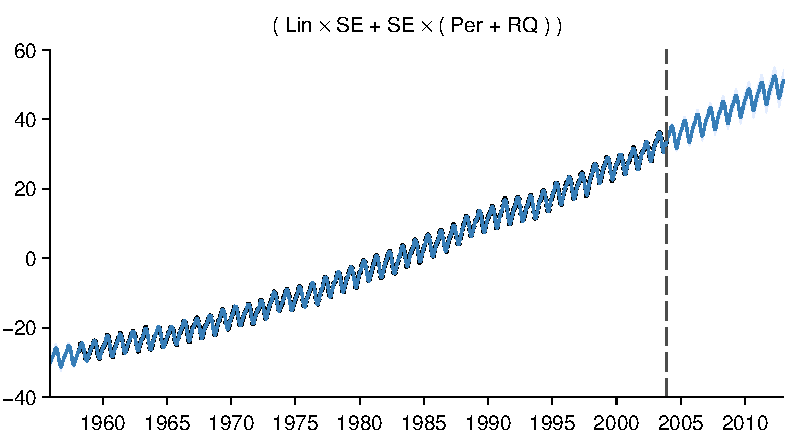
\includegraphics[width=\wmgd,height=\hmgd]{\mdrd/03-mauna2003-s_all} \\ = \\
\mbm 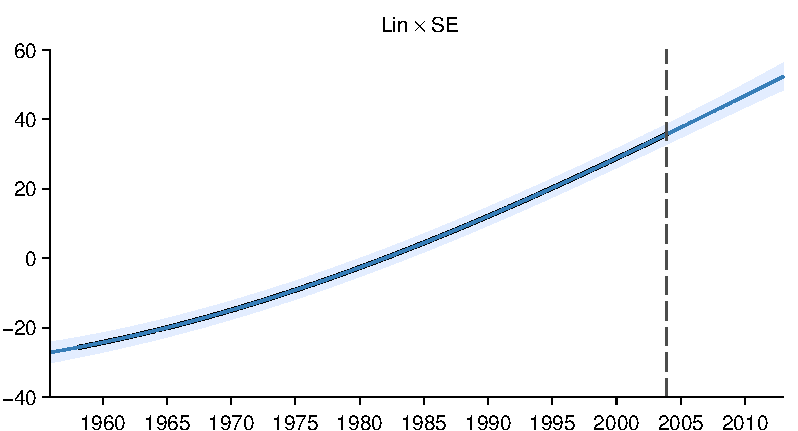
\includegraphics[width=\wmgd,height=\hmgd]{\mdrd/03-mauna2003-s_1} \\ + \\
\mbm 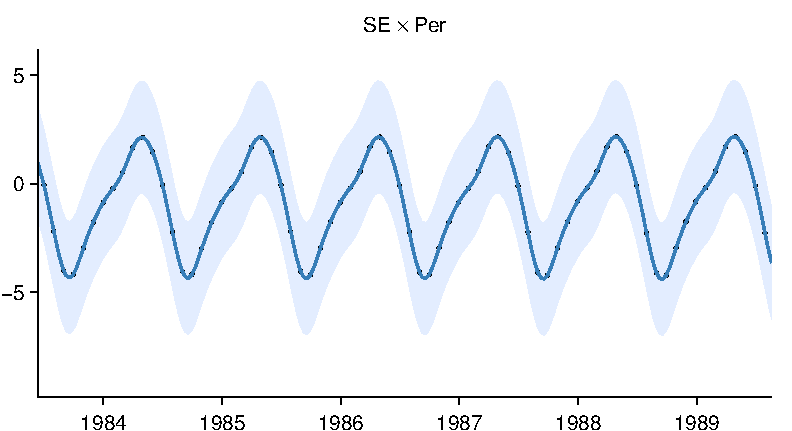
\includegraphics[width=\wmgd,height=\hmgd]{\mdrd/03-mauna2003-s_2_zoom} \\ + \\
\mbm 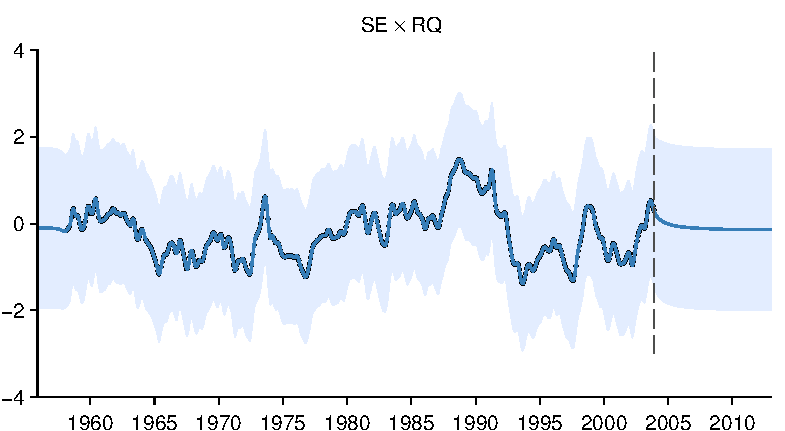
\includegraphics[width=\wmgd,height=\hmgd]{\mdrd/03-mauna2003-s_3} \\ + \\
\mbm 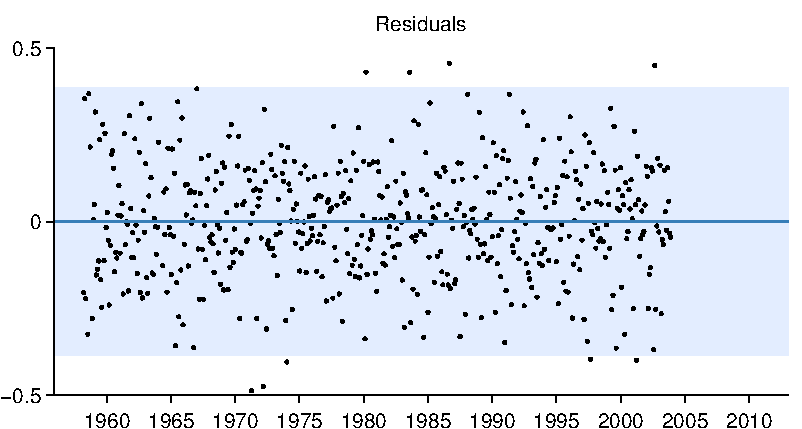
\includegraphics[width=\wmgd,height=\hmgd]{\mdrd/03-mauna2003-s_resid}
\end{tabular}
\caption[Decomposition of the Mauna Loa data.]{First row: The posterior on the Mauna Loa dataset, after a search of depth 10.  Subsequent rows show the automatic decomposition of the time series.  The decompositions shows long-term, yearly periodic, medium-term anomaly components, and residuals, respectively.  In the third row, the scale has been changed in order to clearly show the yearly periodic structure.}
\label{fig:mauna_decomp}
\end{centering}
\end{figure}

Figure \ref{fig:mauna_grow} shows the posterior mean and variance on this dataset as the search depth increases.
While the data can be smoothly interpolated by a single base kernel model, the extrapolations improve dramatically as the increased search depth allows more structure to be included.

Figure \ref{fig:mauna_decomp} shows the final model chosen by our method, together with its decomposition into additive components.
The final model exhibits both plausible extrapolation and interpretable components: a long-term trend, annual periodicity and medium-term correlated deviations; the same components chosen by \citet{Rasmussen2006-ml}.
We also plot the residuals, observing that there is little obvious structure left in the data.  
On this example, our search procedure is able to automate this construction where previously two \gp{} experts devoted 4 pages of text and analysis\footnotemark{} to the development of a composite kernel.
\footnotetext{Admittedly this was intended as teaching material}

\paragraph{Airline passenger data}

Figure \ref{fig:airline_decomp} shows the decomposition produced by applying our method to monthly totals of international airline passengers~\citep[e.g.][]{Box1976-qk}.
We observe similar components to the previous dataset: a long term trend, annual periodicity and medium-term deviations.
In addition, the composite kernel captures the near-linearity of the long-term trend, and the linearly growing amplitude of the annual oscillations.

\paragraph{Solar irradiance Data} 
Finally, we analysed annual solar irradiation data from 1610 to 2011 \citep{Lean1995-vp}.
%
\begin{figure}[ht]
\begin{centering}
\newcommand{\wsd}{0.75\columnwidth}
\newcommand{\hsd}{0.22\columnwidth}
\newcommand{\srd}{\constructionfigsdir/decomposition/11-Feb-02-solar-s}  % solar decomp results dir
\newcommand{\mbs}{\hspace{-0.0cm}}  % move back
\begin{tabular}{c}
\mbs 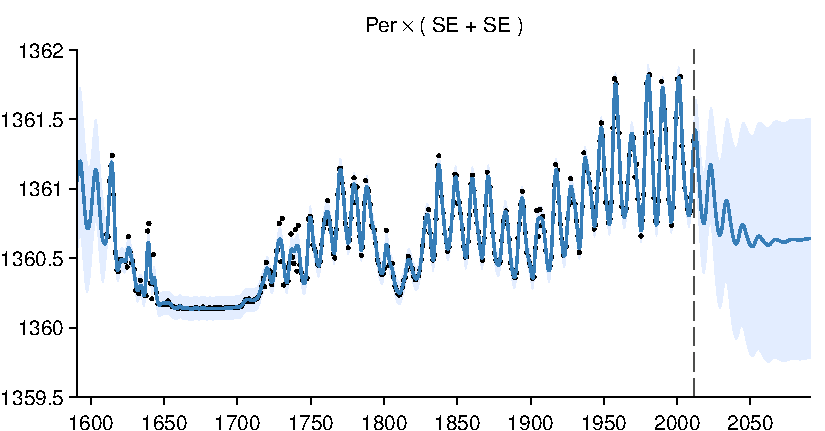
\includegraphics[width=\wsd,height=\hsd]{\srd/02-solar-s_all} \\
\mbs 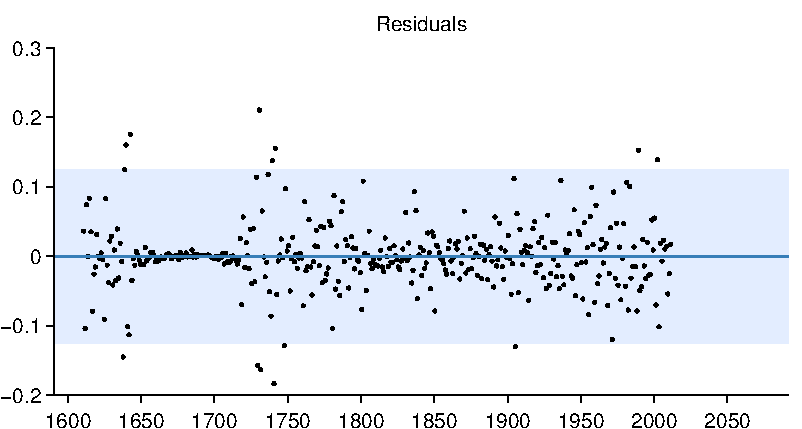
\includegraphics[width=\wsd,height=\hsd]{\srd/02-solar-s_resid}
\end{tabular}
\caption[Posterior and residuals on the solar irradiance data.]{Full posterior and residuals on the solar irradiance dataset.}
\label{fig:solar_decomp}
\end{centering}
\end{figure}
%
The posterior and residuals of the learned kernel are shown in figure \ref{fig:solar_decomp}.
%
\begin{figure}[ht]
\begin{centering}
\newcommand{\wagd}{0.75\columnwidth}
\newcommand{\hagd}{0.22\columnwidth}
\newcommand{\mb}{\hspace{-0.0cm}}  % move back
%\newcommand{\ard}{../figures/decomposition/11-Feb-01-airline-s}  % airline results dir
\newcommand{\ard}{\constructionfigsdir/decomposition/31-Jan-v301-airline-months}  % airline results dir
\begin{tabular}{c}
\mb 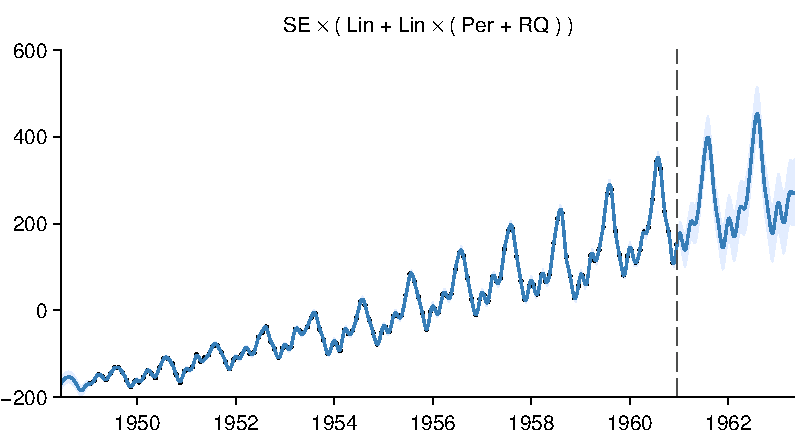
\includegraphics[width=\wagd,height=\hagd]{\ard/01-airline-months_all} \\
 = \\ 
\mb 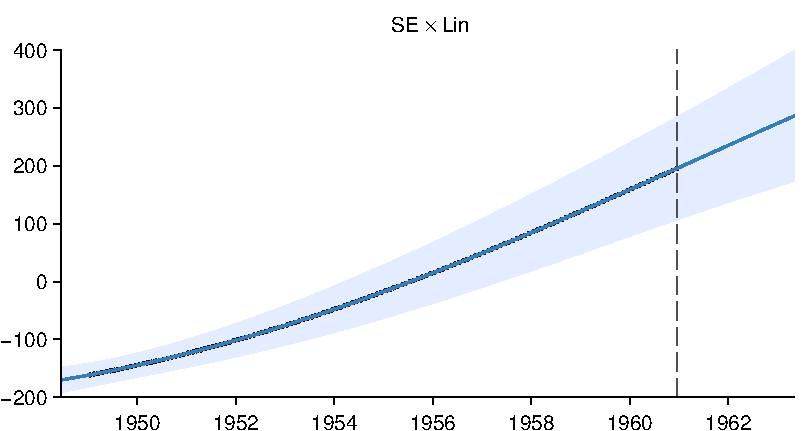
\includegraphics[width=\wagd,height=\hagd]{\ard/01-airline-months_1} \\
 + \\
\mb 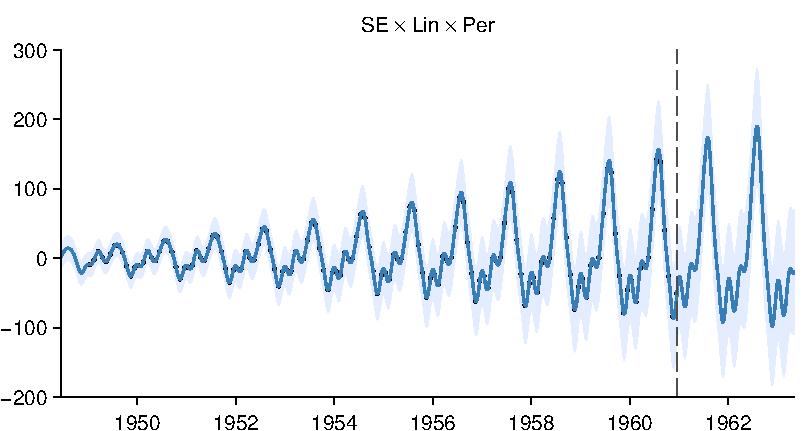
\includegraphics[width=\wagd,height=\hagd]{\ard/01-airline-months_2} \\
 + \\
\mb 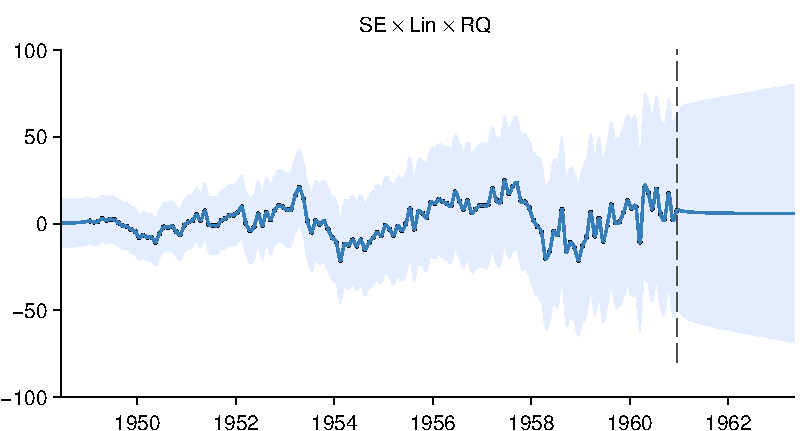
\includegraphics[width=\wagd,height=\hagd]{\ard/01-airline-months_3} \\
 + \\
\mb 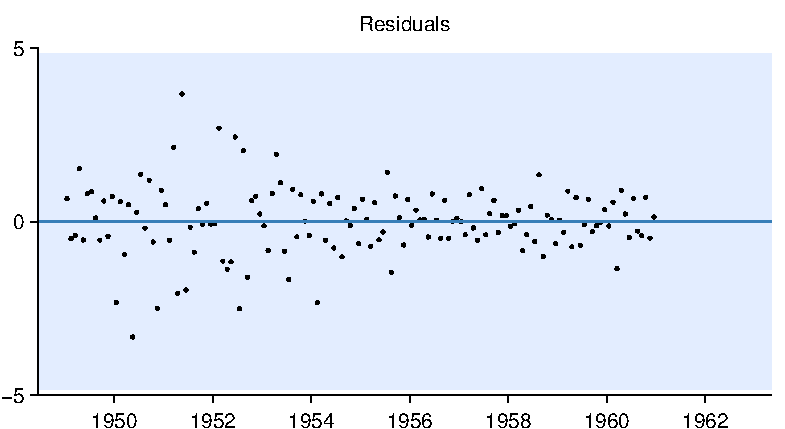
\includegraphics[width=\wagd,height=\hagd]{\ard/01-airline-months_resid}
\end{tabular}
\caption[Decomposition of the airline data.]{First row:  The airline dataset and posterior after a search of depth 10.  Subsequent rows: Additive decomposition of posterior into long-term smooth trend, yearly variation, and short-term deviations.  Due to the linear kernel, the marginal variance grows over time, making this a heteroscedastic model.
}
\label{fig:airline_decomp}
\end{centering}
\end{figure}
%
None of the models in our search space are capable of parsimoniously representing the lack of variation from 1645 to 1715.
Despite this, our approach fails gracefully: the learned kernel still captures the periodic structure, and the quickly growing posterior variance demonstrates that the model is uncertain about long term structure.
In chapter~\ref{ch:description} we demonstrate that an expanded space of kernel families is able to accurately model this phenomenon.

\section{Validation on synthetic data}
\label{sec:synthetic}

\begin{table}[ht!]
\caption[Synthetic validation of kernel search.]{{\small
Kernels chosen by our method on synthetic data generated using known kernel structures. $D$ denotes the dimension of the functions being modelled.  SNR indicates the signal-to-noise ratio. Dashes - indicate no structure.
}}
\label{tbl:synthetic}
\begin{center}
{\small
\begin{tabular}{c c | c c c}
True Kernel & $D$ & SNR = 10 & SNR = 1 & SNR = 0.1 \\
\hline
$\SE + \RQ$                               & 1 
                                              & $\SE$
                                              & $\SE \kerntimes \Per$
                                              & $\SE$
                                              \\
$\Lin \kerntimes \Per$                        & 1 
                                              & $\Lin \kerntimes \Per$
                                              & $\Lin \kerntimes \Per$
                                              & $\SE$
                                              \\
$\SE_1 + \RQ_2$                           & 2 
                                              & $\SE_1 + \SE_2$
                                              & $\Lin_1 + \SE_2$ 
                                              & $\Lin_1$
                                              \\
$\SE_1 + \SE_2 \kerntimes \Per_1 + \SE_3$     & 3 
                                              & $\SE_1 + \SE_2 \kerntimes \Per_1 + \SE_3$
                                              & $\SE_2 \kerntimes \Per_1 + \SE_3$
                                              & -
                                              \\
$\SE_1 \kerntimes \SE_2$                      & 4 
                                              & $\SE_1 \kerntimes \SE_2$
                                              & $\Lin_1 \kerntimes \SE_2$
                                              & $\Lin_2$
                                              \\
$\SE_1 \kerntimes \SE_2 + \SE_2 \kerntimes \SE_3$ & 4 
                                              & $\SE_1 \kerntimes \SE_2 + \SE_2 \kerntimes \SE_3$
                                              & $\SE_1 + \SE_2 \kerntimes \SE_3$
                                              & $\SE_1$
                                              \\
\multirow{2}{*}{$(\SE_1 + \SE_2) \kerntimes (\SE_3 + \SE_4)$} & \multirow{2}{*}{4} 
                                              & $(\SE_1 + \SE_2) \kerntimes \ldots$
                                              & $(\SE_1 + \SE_2) \kerntimes \dots$
                                              & \multirow{2}{*}{-}
                                              \\
                                              &
                                              & $(\SE_3\kerntimes\Lin_3\kerntimes\Lin_1 + \SE_4)$ 
                                              & $\SE_3 \kerntimes \SE_4$                                           
\end{tabular}
}
\end{center}
\end{table}

We validated our method's ability to recover known structure on a set of synthetic datasets.
For several composite kernel expressions, we constructed synthetic data by first sampling 300 points uniformly at random, then sampling function values at those points from a \gp{} distribution.
We then added \iid Gaussian noise to the functions, at various signal-to-noise ratios (SNR).

Table~\ref{tbl:synthetic} lists the true kernels we used to generate the data.
Subscripts indicate which dimension each kernel was applied to.
Subsequent columns show the dimensionality $D$ of the input space, and the kernels chosen by our search for different SNRs.
Dashes - indicate that no kernel had a higher marginal likelihood than modelling the data as \iid Gaussian noise.

For the highest SNR, the method finds all relevant structure in all but one test.
The reported additional linear structure is explainable by the fact that functions sampled from \kSE{} kernels with long length scales occasionally have near-linear trends.
As the noise increases, our method generally backs off to simpler structures.

\section{Quantitative evaluation}
\label{sec:quantitative}

%In addition to producing highly interpretable decompositions of regression functions, our method also produces state of the art predictions in both extrapolation and interpolation tasks.
In addition to the qualitative evaluation above, we investigated quantitatively how our method performs on both extrapolation and interpolation tasks.

\subsection{Extrapolation}

\begin{figure}
\centering
\begin{tabular}{c}
\hspace{-0.0cm} 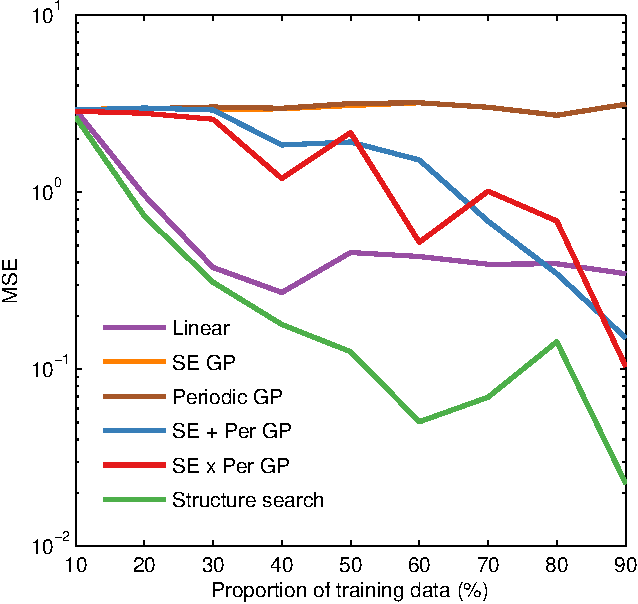
\includegraphics[width=0.8\columnwidth]{\constructionfigsdir/extrapolation_curves/01-airline-s-ex-curve_hint.pdf}
\end{tabular}
\caption[Extrapolation performance on the airline dataset.]{Extrapolation performance on the airline dataset.  We plot test-set MSE as a function of the fraction of the dataset used for training. 
}
\label{fig:extrapolation}
\end{figure}

We compared the extrapolation capabilities of our model against standard baselines\footnotemark.
Dividing the airline dataset into contiguous training and test sets, we computed the predictive mean-squared-error (MSE) of each method.
We varied the size of the training set from the first 10\% to the first 90\% of the data.

Figure \ref{fig:extrapolation} shows the learning curves of linear regression, a variety of fixed kernel family \gp{} models, and our method.  
\gp{} models with only \kSE{} and \kPer{} kernels did not capture the long-term trends, since the best parameter values in terms of \gp{} marginal likelihood only capture short term correlations. 
Linear regression approximately captured the long-term trend, but quickly plateaued in predictive performance.
The more richly structured \gp{} models (${\kSE + \kPer}$ and ${\kSE \times \kPer}$) eventually captured more structure and performed better, but the full structures discovered by our search outperformed the other approaches in terms of predictive performance for all data amounts.
We perform a more extensive version of this experiment in chapter~\ref{ch:description}.

\footnotetext{
In one dimension, the predictive means of all baseline methods in table \ref{tbl:Regression Mean Squared Error} are identical to that of a \gp{} with an $\kSE{}$ kernel.}

\subsection{High-dimensional prediction}

To evaluate the predictive accuracy of our method in a high-dimensional setting, we extended the comparison of \cite{Duvenaud2011-wb} to include our method.
We performed 10 fold cross validation on 5 datasets\footnotemark{} comparing 5 methods in terms of mean squared error and predictive likelihood.
Our kernel search procedure was run up to depth 10, using the \SE{} and \RQ{} base kernel families\footnotemark{}.
\footnotetext{We did not believe a priori to find any periodicity or perfect linearity in these data sets}

\footnotetext{The data sets had dimensionalities ranging from 4 to 13, and the number of data points ranged from 150 to 450.} 

The comparison included three methods with fixed kernel families: Additive \gp{}s, Generalized Additive Models (GAM), and a \gp{} with a standard \kSE{} kernel using Automatic Relevance Determination (\gp{} \kSE{}-ARD). 
Also included was the related kernel-search method of Hierarchical Kernel Learning (HKL).

Results are presented in tables \ref{tbl:Regression Mean Squared Error} and \ref{tbl:Regression Negative Log Likelihood}.
Our method outperformed the next-best method in each test, although not substantially.

\begin{table}[ht]
\caption[MSE comparison of kernel search and related algorithms.]{{\small
Comparison of multidimensional regression performance in terms of cross validated mean squared error. Bold results are not significantly different from the best-performing method in each experiment, in a paired t-test with a $p$-value of 5\%.
}}
\label{tbl:Regression Mean Squared Error}
\begin{center}
\begin{tabular}{l | r r r r r}
Method & \rotatebox{0}{ bach  }  & \rotatebox{0}{ concrete  }  & \rotatebox{0}{ puma }  & \rotatebox{0}{ servo }  & \rotatebox{0}{ housing }  \\ \hline
Linear Regression & $1.031$ & $0.404$ & $0.641$ & $0.523$ & $0.289$ \\
GP GAM & $1.259$ & $0.149$ & $0.598$ & $0.281$ & $0.161$ \\
HKL & $\mathbf{0.199}$ & $0.147$ & $0.346$ & $0.199$ & $0.151$ \\
GP Squared-exp & $\mathbf{0.045}$ & $0.157$ & $\mathbf{0.317}$ & $\mathbf{0.126}$ & $\mathbf{0.092}$ \\
GP Additive & $\mathbf{0.045}$ & $\mathbf{0.089}$ & $\mathbf{0.316}$ & $\mathbf{0.110}$ & $0.102$ \\
\hline
Kernel search & $\mathbf{0.044}$ & $\mathbf{0.087}$ & $\mathbf{0.315}$ & $\mathbf{0.102}$ & $\mathbf{0.082}$ \\
\end{tabular}
\end{center}
\end{table}

\begin{table}[ht]
\caption[Likelihood comparison of kernel search and related algorithms.]{{\small
Comparison of multidimensional regression performance in terms of cross validated negative log likelihood. Bold results are not significantly different from the best-performing method in each experiment, in a paired t-test with a $p$-value of 5\%.
}}
\label{tbl:Regression Negative Log Likelihood}
\begin{center}
\begin{tabular}{l | r r r r r}
Method & \rotatebox{0}{ bach  }  & \rotatebox{0}{ concrete  }  & \rotatebox{0}{ puma }  & \rotatebox{0}{ servo }  & \rotatebox{0}{ housing }  \\ \hline
Linear Regression & $2.430$ & $1.403$ & $1.881$ & $1.678$ & $1.052$ \\
GP GAM & $1.708$ & $0.467$ & $1.195$ & $0.800$ & $0.457$ \\
GP Squared-exp & $\mathbf{-0.131}$ & $0.398$ & $\mathbf{0.843}$ & $0.429$ & $0.207$ \\
GP Additive & $\mathbf{-0.131}$ & $\mathbf{0.114}$ & $\mathbf{0.841}$ & $\mathbf{0.309}$ & $0.194$ \\
\hline
Kernel search & $\mathbf{-0.141}$ & $\mathbf{0.065}$ & $\mathbf{0.840}$ & $\mathbf{0.265}$ & $\mathbf{0.059}$ \\
\end{tabular}
\end{center}
\end{table}

All \gp{} kernel parameter estimation was performed by automated calls to the GPML toolbox\footnote{Available at 
\href{http://www.gaussianprocess.org/gpml/code/}
{\texttt{www.gaussianprocess.org/gpml/code/}}
}; Python code to perform all experiments is available on github\footnote{
\href{http://www.github.com/jamesrobertlloyd/gp-structure-search}
{\texttt{github.com/jamesrobertlloyd/gp-structure-search}}
}.

\section{Discussion}
\label{sec:construction:discussion}

Towards the goal of automating the choice of kernel family, we introduced a space of composite kernels defined compositionally as sums and products of a small number of base kernels.  
The set of models in this space includes many standard regression models.
We proposed a search procedure for this space of kernels which parallels human model building strategies.

We found that the learned structures are often capable of accurate extrapolation in complex time-series datasets, and are competitive with widely used kernel classes and kernel combination methods on a variety of prediction tasks.
The learned kernels often yield decompositions of a signal into diverse and interpretable components, enabling visual model criticism of complex nonparametric models.
We believe that a data-driven approach to choosing kernel structures automatically can help make nonparametric regression and classification methods accessible to non-experts.

However, there are a number of improvements that could be made to the procedure described in this chapter.
Some of those improvements are implemented in the work described in chapter~\ref{ch:description} but we now discuss two other shortcomings and discuss potential future work to overcome them.

\subsection{Estimating marginal likelihoods}

In section~\ref{sec:construction:search} it was stated that we used the Bayesian information criterion (BIC) \citep{Schwarz1978-wp} to approximate the model evidence of a kernel family.
The model evidence is a central quantity in this work since it allows us to balance model complexity and model fit in order to find a parsimonious explanation of a data set.
However, the technical conditions required for a completely sound usage of BIC are not met by the Gaussian process models considered in this chapter.
We now discuss more principled alternatives and the difficulties that remain before they can be applied.

In an exact and fully Bayesian approach we would put priors over the kernel parameters and compute the model evidence of the kernel families with all the parameters integrated out.
Since the relevant equations of Bayes' rule are analytically intractable in this case we turn to approximate inference techniques.
The majority of approximate inference methods taking a fully Bayesian approach to Gaussian process regression have focused on producing approximate samples from the posterior distribution \citep[e.g.][]{Murray2010-hv, Lloyd2012-sb, Snoek2012-ri} but have ignored the estimation of the model evidence.
Variational Bayes and expectation propagation methods naturally produce an estimate or lower bound of model evidence and have been applied to Gaussian processes \citep[e.g.][]{Rasmussen2006-ml, Hensman2013-ox}.
However, to the best of my knowledge, all existing techniques condition on kernel parameters which are then optimised which means we are still faced with the problem of appropriately penalising our optimisation of a growing number of kernel parameters.
While there is a growing literature on generic and automatic methods for approximating model evidences \citep[e.g.][]{Skilling2006-ez, Gerrish_undated-zh, Feroz2013-dj} I am unaware of successful applications of these techniques to Gaussian processes with unknown kernel parameters.

A simple method that we attempted to utilise was the Laplace approximation to the model evidence \citep[e.g.][]{Bishop2006-yy}.
This method approximates the log-likelihood function as a quadratic with centre at a mode of the likelihood and curvature at the mode matched to that of the true log-likelihood.
To be able to calculate this approximation one must be sufficiently close to a mode of the likelihood in order to be able to produce a numerical estimate of the curvature that is strictly negative definite (\ie defining an appropriate turning point of the likelihood).

The situation of not quite being at the mode however is not just a numerical annoyance, it is becoming increasingly common.
We found that the conjugate gradients solver used within the kernel search algorithm could become confused by numerical noise and would terminate before it reached a mode.
Also, as data sets become increasingly large and computation and time constraints of algorithms become increasingly important it will often be irrational to run optimisers to completion since it may be more beneficial to spend computation on investigating other models \citep[e.g.][]{Swersky2014-aw}.

A potential way forward is to imagine a more general version of the Laplace approximation.
The Laplace approximation attempts to approximate the log-likelihood with a quadratic; this can be achieved without exactly having found the mode simply by performing regression using a quadratic regression function.
This could be viewed as a simple version of Bayesian quadrature \citep[e.g.][]{Ghahramani2002-by, OHagan1991-wg} with potentially attractive computation time.
A full analysis of this idea would also likely interact with recent reinterpretations of classic optimisation algorithms as approximate inference in probabilistic models \citep[e.g.][]{Hennig2012-wv}.

\subsection{Model selection rather than model averaging}

In this chapter we have demonstrated that selecting the model with the highest model evidence encountered along the search was sufficient to achieve good empirical performance on the moderate dimensional datasets considered.
However, much like BIC guided linear model selection will fail on high dimensional problems \citep[e.g.][]{Hastie2009-hj}, so will the kernel search as currently described.
Staying within the Bayesian paradigm it is conceptually simple to alleviate this problem by instead computing a Bayes model average \citep[e.g.][]{Hoeting1999-tn} over kernel families.
The natural search objective would then change from optimising the model evidence of a single kernel family to that of the sum of model evidences of all kernel families visited by the search, appropriately weighted by a prior over kernel families.

\outbpdocument{
\bibliographystyle{plainnat}
\bibliography{references.bib}
}
